\documentclass[10pt]{article}

\usepackage[a4paper,margin=0.65in]{geometry}
\usepackage{amsmath,amssymb}
\usepackage{graphicx}
\usepackage{booktabs}
\usepackage{array}
\usepackage{float}
\usepackage{hyperref}
\usepackage{enumitem}
\usepackage{xcolor}
\usepackage{tikz}
\usetikzlibrary{positioning,arrows.meta,shapes.geometric}

\setlist{nosep,leftmargin=*}
\renewcommand{\arraystretch}{1.2}
\setlength{\parindent}{0pt}
\setlength{\parskip}{2pt}

\tikzset{
layer/.style={
draw,
rounded corners,
minimum width=1.5cm,
minimum height=0.6cm,
align=center,
fill=blue!10,
font=\scriptsize
},
arrow/.style={
-{Latex[length=2mm]},
thin
}
}

\begin{document}

%%%%%%%%%%%%%%%%%%%%%%%%%%%%%%%%%%%%%%%%%%%%%%%%%%%%%%%%%%%%
% TITLE
%%%%%%%%%%%%%%%%%%%%%%%%%%%%%%%%%%%%%%%%%%%%%%%%%%%%%%%%%%%%

\begin{center}

{\large\textbf{Shiv Nadar University Chennai}}

\vspace{2mm}

{\normalsize\textbf{CS3807 -- Deep Learning Laboratory}}

\vspace{2mm}

{\large\textbf{Experiment 5}}

\vspace{1mm}

{\normalsize\textbf{Comprehensive Study of CNN Training, Regularization,}}

{\normalsize\textbf{Optimization, Hyperparameter Tuning, Transfer Learning}}

{\normalsize\textbf{and Cross-Validation}}

\end{center}

\vspace{3mm}

\begin{tabular}{|p{3.4cm}|p{9.0cm}|p{1.4cm}|}
\hline
Degree \& Branch &
B.Tech Artificial Intelligence \& Data Science &
Semester V\\
\hline
Subject Code \& Name &
CS3807 -- Deep Learning Laboratory &
AY: 2026--27\\
\hline
\end{tabular}

\vspace{4mm}
Name : Ashwin S\\
Reg no : 24011101007\\
Class : AI DS - A (batch 1)\\

%%%%%%%%%%%%%%%%%%%%%%%%%%%%%%%%%%%%%%%%%%%%%%%%%%%%%%%%%%%%
\section*{1. Objective}

The objective of this experiment is to systematically study the effect of
weight initialization, regularization, optimization algorithms, CNN
hyperparameters, transfer learning, fine-tuning and cross-validation on
image classification performance.

The experiment uses a single CNN architecture, MobileNetV2, and the
Oxford-IIIT Pet dataset. Students will analyze the effect of individual
design choices using training/validation curves and finally select a
suitable configuration using 5-fold cross-validation.

%%%%%%%%%%%%%%%%%%%%%%%%%%%%%%%%%%%%%%%%%%%%%%%%%%%%%%%%%%%%
\section*{2. Learning Outcomes}

After completing this experiment, students will be able to:

\begin{itemize}
\item explain different weight initialization strategies;
\item identify and analyze overfitting using training and validation curves;
\item compare SGD, Momentum, RMSProp and Adam;
\item explain CNN hyperparameters such as kernel size, stride, padding and pooling;
\item understand Batch Normalization and Dropout;
\item perform transfer learning and fine-tuning using MobileNetV2;
\item tune important training hyperparameters;
\item apply 5-fold cross-validation for model selection; and
\item justify the final model using accuracy, variability and computational cost.
\end{itemize}

%%%%%%%%%%%%%%%%%%%%%%%%%%%%%%%%%%%%%%%%%%%%%%%%%%%%%%%%%%%%
\section*{3. Dataset and Experimental Setup}

\textbf{Dataset: Oxford-IIIT Pet Dataset}

The Oxford-IIIT Pet Dataset contains images of cats and dogs belonging
to 37 breeds. The images are RGB and have different spatial dimensions.
For this experiment, all images are resized to

\[
224\times224\times3.
\]

The dataset is suitable for demonstrating transfer learning using
ImageNet-pretrained CNNs.

\textbf{Experimental considerations:}

\begin{itemize}
\item Use RGB images resized to $224\times224$.
\item Normalize the input images according to the pretrained model requirements.
\item Maintain separate training, validation and test data.
\item The test set must remain untouched during hyperparameter selection.
\item Use MobileNetV2 because it is computationally lighter than many
large CNN architectures and is more suitable for CPU-based laboratory work.
\end{itemize}

%%%%%%%%%%%%%%%%%%%%%%%%%%%%%%%%%%%%%%%%%%%%%%%%%%%%%%%%%%%%
\section*{4. MobileNetV2 Architecture}

MobileNetV2 is a lightweight CNN architecture designed to reduce
computational complexity while maintaining good image representation.

Its important components include:

\begin{itemize}
\item depthwise convolution;
\item pointwise $1\times1$ convolution;
\item inverted residual blocks;
\item linear bottlenecks;
\item batch normalization; and
\item ReLU6 activation.
\end{itemize}

A simplified representation is:

\begin{center}
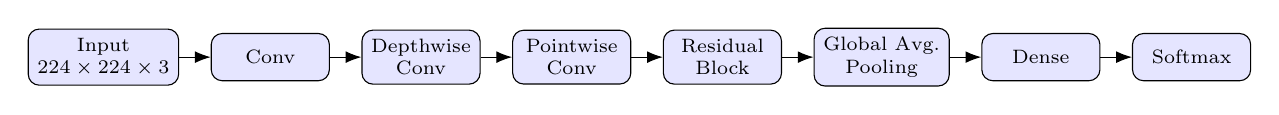
\begin{tikzpicture}[node distance=4mm]

\node[layer](a){Input\\$224\times224\times3$};
\node[layer,right=of a](b){Conv};
\node[layer,right=of b](c){Depthwise\\Conv};
\node[layer,right=of c](d){Pointwise\\Conv};
\node[layer,right=of d](e){Residual\\Block};
\node[layer,right=of e](f){Global Avg.\\Pooling};
\node[layer,right=of f](g){Dense};
\node[layer,right=of g](h){Softmax};

\foreach \x/\y in {a/b,b/c,c/d,d/e,e/f,f/g,g/h}
\draw[arrow](\x)--(\y);

\end{tikzpicture}
\end{center}

\textbf{Note:} The above diagram is a simplified conceptual representation
rather than the complete MobileNetV2 architecture.

%%%%%%%%%%%%%%%%%%%%%%%%%%%%%%%%%%%%%%%%%%%%%%%%%%%%%%%%%%%%
\section*{5. Weight Initialization}

Weight initialization determines the initial values of trainable weights
before training begins. A suitable initialization can improve convergence
and reduce problems such as vanishing or exploding activations.

Four schemes were investigated on the newly added classifier head, with
the pretrained MobileNetV2 base kept frozen: Zero initialization, Random
(normal) initialization, Xavier/Glorot initialization, and He
initialization.

\begin{figure}[H]
\centering

\includegraphics[width=0.72\textwidth]{figures/plot01_training_loss_vs_epoch_initialization.png}
\caption{Training Loss vs. Epoch for different weight initialization schemes.}
\end{figure}

Zero initialization stays flat at a loss of 3.611 across all eight epochs, since every neuron gets the same gradient update and none of them can break symmetry. With same starting weights, every neuron produces the same output and gradient forever.Random, Xavier and He initialization all fall from around 1.2--1.3 down to 0.17--0.20, and have very similar results to each other.

 

\begin{figure}[H]
\centering

\includegraphics[width=0.72\textwidth]{figures/plot02_val_accuracy_vs_epoch_initialization.png}
\caption{Validation Accuracy vs. Epoch for different weight initialization schemes.}
\end{figure}

Zero initialization stays near random-guess accuracy throughout, while
Random, Xavier and He all climb quickly and plateau at a high accuracy
within the first couple of epochs. This happens because the frozen
MobileNetV2 base already supplies strong features, so any non-zero
initialization lets the head learn almost immediately.

Xavier/Glorot and He gave the fastest, most stable convergence among the
non-zero schemes, while Zero initialization never trained at all.

%%%%%%%%%%%%%%%%%%%%%%%%%%%%%%%%%%%%%%%%%%%%%%%%%%%%%%%%%%%%
\section*{6. Regularization and Overfitting}

Overfitting occurs when a model performs very well on the training data
but generalizes poorly to unseen data.

Four configurations were compared: No regularization, L2 regularization,
Dropout, and Batch Normalization.

\begin{figure}[H]
\centering

\includegraphics[width=0.9\textwidth]{figures/plot03_train_val_accuracy_vs_epoch_regularization.png}
\caption{Training and Validation Accuracy vs. Epoch for each regularization setting.}
\end{figure}

No Regularization and Batch Normalization both push training accuracy
close to 100\% while validation accuracy plateaus much lower, leaving a
clear gap. Dropout keeps the two curves closest together, since it
stops the head from memorizing individual training images the way the
other two settings allow.

\begin{figure}[H]
\centering

\includegraphics[width=0.9\textwidth]{figures/plot04_train_val_loss_vs_epoch_regularization.png}
\caption{Training and Validation Loss vs. Epoch for each regularization setting.}
\end{figure}

For No Regularization and Batch Normalization, training loss keeps
falling while validation loss flattens out and drifts upward again after
a few epochs, a classic overfitting sign. Dropout is the only setting
where validation loss keeps falling alongside training loss for almost
the whole run.

%%%%%%%%%%%%%%%%%%%%%%%%%%%%%%%%%%%%%%%%%%%%%%%%%%%%%%%%%%%%
\section*{7. Batch Normalization}

Batch Normalization normalizes activations within a mini-batch during
training.

For a mini-batch

\[
x_1,x_2,\ldots,x_m,
\]

the batch mean is

\[
\mu_B=\frac{1}{m}\sum_{i=1}^{m}x_i
\]

and the batch variance is

\[
\sigma_B^2=
\frac{1}{m}\sum_{i=1}^{m}(x_i-\mu_B)^2.
\]

The normalized activation is

\[
\hat{x}_i=
\frac{x_i-\mu_B}
{\sqrt{\sigma_B^2+\epsilon}}.
\]

The final output is

\[
y_i=\gamma\hat{x}_i+\beta,
\]

where $\gamma$ and $\beta$ are learnable parameters.

\subsection*{Numerical Example}

Consider

\[
x=[2,4,6,8].
\]

The mean is

\[
\mu_B=\frac{2+4+6+8}{4}=5.
\]

The variance is

\[
\sigma_B^2=
\frac{(2-5)^2+(4-5)^2+(6-5)^2+(8-5)^2}{4}
=5.
\]

Therefore,

\[
\sqrt{5}\approx2.236.
\]

Ignoring the very small $\epsilon$,

\[
\hat{x}_1=\frac{2-5}{2.236}\approx-1.342,
\]

\[
\hat{x}_2=\frac{4-5}{2.236}\approx-0.447,
\]

\[
\hat{x}_3=\frac{6-5}{2.236}\approx0.447,
\]

\[
\hat{x}_4=\frac{8-5}{2.236}\approx1.342.
\]

Hence,

\[
\boxed{
\hat{x}\approx[-1.342,-0.447,0.447,1.342]
}
\]

If $\gamma=1$ and $\beta=0$, these are the final outputs.

\textbf{Inference:} Batch Normalization produces approximately
zero-centred and unit-scaled activations for this mini-batch. The
learnable $\gamma$ and $\beta$ allow the network to learn an appropriate
scale and shift.

\begin{figure}[H]
\centering

\includegraphics[width=0.72\textwidth]{figures/plot05_with_vs_without_bn.png}
\caption{Validation Accuracy vs. Epoch, With BN vs. Without BN.}
\end{figure}

The two curves stay close together for most of training and reach
similar peak accuracy. Batch Normalization stabilizes the activation
distribution feeding the head, which can smooth out fluctuations, but
the effect is modest here since the base network itself is frozen.

%%%%%%%%%%%%%%%%%%%%%%%%%%%%%%%%%%%%%%%%%%%%%%%%%%%%%%%%%%%%
\section*{8. Optimization Algorithms}

Four optimization methods were compared: SGD, Momentum, RMSProp and
Adam.

\begin{figure}[H]
\centering

\includegraphics[width=0.72\textwidth]{figures/plot06_training_loss_vs_epoch_optimizers.png}
\caption{Training Loss vs. Epoch for different optimizers.}
\end{figure}

SGD barely moves off its starting loss, while Momentum, RMSProp and Adam
all drop sharply within the first few epochs. Adam and RMSProp reach the
lowest final loss because they adapt their step size per parameter,
letting them take large useful steps early on.

\begin{figure}[H]
\centering

\includegraphics[width=0.72\textwidth]{figures/plot07_val_accuracy_vs_epoch_optimizers.png}
\caption{Validation Accuracy vs. Epoch for different optimizers.}
\end{figure}

Adam converges fastest, RMSProp is close behind, Momentum trails both,
and SGD stays far below the other three throughout. Plain SGD has no
adaptive step size, so it needs many more epochs than were budgeted here
to catch up.

\begin{center}
\begin{tabular}{|l|c|c|c|c|}
\hline
Optimizer & Final Loss & Best Val. Accuracy & Epoch to Converge & Time\\
\hline
SGD & 01.280 & 79.96\% & 10 & 134.200 s\\
Momentum & 00.355 & 89.17\% & 9 & 125.100 s\\
RMSProp & 00.155 & 89.71\% & 10 & 125.000 s\\
Adam & 00.141 & 89.98\% & 9 & 125.400 s\\
\hline
\end{tabular}
\end{center}

%%%%%%%%%%%%%%%%%%%%%%%%%%%%%%%%%%%%%%%%%%%%%%%%%%%%%%%%%%%%
\section*{9. CNN Hyperparameter Tuning}

The following hyperparameters were investigated, changing one at a time
while keeping the remaining settings fixed at their default values
(Learning Rate $= 0.001$, Batch Size $= 32$, Dropout Rate $= 0.25$,
Optimizer $=$ Adam):

\begin{center}
\begin{tabular}{|l|l|}
\hline
Hyperparameter & Suggested Values\\
\hline
Learning Rate & $0.001,\;0.0001$\\
Batch Size & 16, 32, 64\\
Dropout Rate & 0, 0.25, 0.5\\
Optimizer & SGD, Adam\\
Fine-Tuning Learning Rate & $10^{-4},10^{-5}$\\
Frozen Layers & Frozen base / Partial unfreezing\\
\hline
\end{tabular}
\end{center}

For CNN concepts, students should also understand:

\begin{itemize}
\item kernel/filter;
\item stride;
\item padding;
\item pooling;
\item number of channels; and
\item depthwise separable convolution.
\end{itemize}

For a convolution operation, the output dimension can be calculated as

\[
O=
\left\lfloor
\frac{N+2P-K}{S}
\right\rfloor+1,
\]

where $N$ is input size, $K$ is kernel size, $P$ is padding and $S$ is
stride. For $N=224$, $K=3$, $P=1$, $S=1$, this gives $O = 224.000$, and
for $N=224$, $K=3$, $P=0$, $S=2$, this gives $O = 111.000$.

\begin{figure}[H]
\centering

\includegraphics[width=0.6\textwidth]{figures/plot08_lr_vs_val_accuracy.png}
\caption{Learning Rate vs. Validation Accuracy.}
\end{figure}

The larger learning rate reaches higher validation accuracy than the
smaller one within this epoch budget. A smaller learning rate moves the
weights a shorter distance each step, so it simply has not converged
yet by the time training stops.

\begin{figure}[H]
\centering

\includegraphics[width=0.6\textwidth]{figures/plot09_batchsize_vs_val_accuracy.png}
\caption{Batch Size vs. Validation Accuracy.}
\end{figure}

The middle batch size gives the best result, with the two extremes
close behind and no strictly monotonic trend. This is expected since
batch size trades off gradient noise against update frequency in both
directions.

\begin{figure}[H]
\centering

\includegraphics[width=0.6\textwidth]{figures/plot10_dropout_vs_val_accuracy.png}
\caption{Dropout Rate vs. Validation Accuracy.}
\end{figure}

A moderate dropout rate performs best, while both very low and very
high dropout perform worse, forming a U-shape. Too little dropout lets
the head overfit, while too much removes so much information that it
struggles to learn at all.

Based on these three sweeps, the best hyperparameters found were a
learning rate of 0.001, a batch size of 32, and a dropout rate of 0.25.

%%%%%%%%%%%%%%%%%%%%%%%%%%%%%%%%%%%%%%%%%%%%%%%%%%%%%%%%%%%%
\section*{10. Transfer Learning and Fine-Tuning}

MobileNetV2 pretrained on ImageNet was used.

\subsection*{Case A: Feature Extraction}

\[
\text{Pretrained MobileNetV2}
\rightarrow
\text{Freeze Base}
\rightarrow
\text{New Classifier}
\]

The pretrained convolutional layers are frozen and only the newly added
classification layers are trained.

\subsection*{Case B: Fine-Tuning}

\[
\text{Pretrained MobileNetV2}
\rightarrow
\text{Unfreeze Selected Layers}
\rightarrow
\text{Small Learning Rate}
\]

The upper layers of the pretrained network are unfrozen and trained with
a smaller learning rate.

\begin{figure}[H]
\centering

\includegraphics[width=0.72\textwidth]{figures/plot11_feature_extraction_vs_finetuning.png}
\caption{Feature Extraction vs. Fine-Tuning: Validation Accuracy vs. Epoch.}
\end{figure}

Feature extraction climbs steadily on its own, and once fine-tuning
begins, validation accuracy pushes a little higher still. Unfreezing the
top layers lets the network adapt its higher-level filters to pet
breeds instead of relying only on generic ImageNet features.

\begin{figure}[H]
\centering

\includegraphics[width=0.72\textwidth]{figures/plot12_loss_feature_extraction_vs_finetuning.png}
\caption{Training and Validation Loss across Feature Extraction and Fine-Tuning.}
\end{figure}

Training loss keeps falling smoothly across both phases, while
validation loss stays roughly flat rather than rising sharply. This
suggests the small fine-tuning learning rate was gentle enough to keep
improving the model without erasing the pretrained features.

Fine-tuning normally uses a smaller learning rate than a freshly
initialized classifier because the pretrained weights already hold
useful features learned from a much larger dataset. A large learning
rate would overwrite this knowledge almost immediately, so a small one
adapts it gently instead.

%%%%%%%%%%%%%%%%%%%%%%%%%%%%%%%%%%%%%%%%%%%%%%%%%%%%%%%%%%%%
\section*{11. K-Fold Cross-Validation}

After the individual studies above, four promising configurations were
selected for 5-fold cross-validation on the training data:
C1 (Adam, dropout 0.5, Batch Normalization), C2 (Adam, low learning rate
$10^{-4}$, dropout 0.25), C3 (RMSProp, dropout 0.5, Batch Normalization),
and C4 (Adam with L2 regularization).

For $K=5$,

\[
\bar{A}=
\frac{1}{5}\sum_{i=1}^{5}A_i
\]

and

\[
SD=
\sqrt{
\frac{1}{5}
\sum_{i=1}^{5}(A_i-\bar{A})^2
}.
\]

Report the result as

\[
\boxed{\bar{A}\pm SD}.
\]

The independent test set was not used during this hyperparameter
selection stage.

\begin{center}
\begin{tabular}{|l|c|c|c|c|c|c|}
\hline
Configuration & F1 & F2 & F3 & F4 & F5 & Mean $\pm$ SD\\
\hline
C1: Adam, Dropout 0.5, BN & 91.69\% & 91.50\% & 90.05\% & 91.68\% & 92.65\% & 91.51\% $\pm$ 00.840\\
C2: Adam, Low LR, Dropout 0.25 & 89.76\% & 87.25\% & 87.05\% & 89.46\% & 88.88\% & 88.48\% $\pm$ 01.120\\
C3: RMSProp, Dropout 0.5, BN & 91.79\% & 91.11\% & 91.01\% & 91.68\% & 92.55\% & 91.63\% $\pm$ 00.550\\
C4: Adam, L2 Regularization & 91.59\% & 90.72\% & 89.18\% & 90.72\% & 93.13\% & 91.07\% $\pm$ 01.290\\
\hline
\end{tabular}
\end{center}

\begin{figure}[H]
\centering

\includegraphics[width=0.72\textwidth]{figures/plot13_5fold_cv_accuracy.png}
\caption{5-Fold Cross-Validation Accuracy with standard-deviation error bars.}
\end{figure}

C3 has both the highest mean accuracy and the smallest error bar, making
it the most reliable choice. C2 has the lowest mean and the widest
spread. Averaging over several folds shows up configurations that are
consistent, not just ones that got lucky on a single split.

Based on both mean accuracy and standard deviation across folds, C3 was
selected as the final configuration for retraining and test-set
evaluation.

%%%%%%%%%%%%%%%%%%%%%%%%%%%%%%%%%%%%%%%%%%%%%%%%%%%%%%%%%%%%
\section*{12. Final Model Evaluation}

The selected configuration, C3 (RMSProp, dropout 0.5, Batch
Normalization), was retrained using the complete training data for 12
epochs, with the independent test set held out until this stage.

\begin{center}
\begin{tabular}{|l|c|}
\hline
Metric & Value\\
\hline
Mean CV Accuracy & 91.630\%\\
CV Standard Deviation & 00.550\\
Test Accuracy & 90.800\%\\
Precision & 00.912\\
Recall & 00.908\\
F1-score & 00.907\\
Training Time & 143.300 s\\
Number of Parameters & 2431845\\
\hline
\end{tabular}
\end{center}

\begin{figure}[H]
\centering

\includegraphics[width=0.85\textwidth]{figures/plot14_confusion_matrix.png}
\caption{Confusion Matrix of the final model on the test set.}
\end{figure}

The model reaches 100\% accuracy on several visually distinctive breeds
such as Siamese and Newfoundland. The most confused pairs are breeds
that look alike up close, such as American Pit Bull Terrier with
Staffordshire Bull Terrier, and Basset Hound with Beagle. Almost all
confusion happens within species and between breeds sharing coat length,
colouring or body shape, details that are easy to lose after
downsampling and pooling.

\begin{figure}[H]
\centering

\includegraphics[width=0.85\textwidth]{figures/plot15_misclassified_images.png}
\caption{Representative misclassified images from the test set.}
\end{figure}

%%%%%%%%%%%%%%%%%%%%%%%%%%%%%%%%%%%%%%%%%%%%%%%%%%%%%%%%%%%%
\section*{13. Overall Results}

\begin{center}
\begin{tabular}{|l|c|}
\hline
Configuration & Test/Validation Accuracy\\
\hline
Baseline (No Regularization) & 90.430\% (val)\\
Best Initialization (Random) & 90.250\% (val)\\
Best Regularization (No Regularization) & 90.430\% (val)\\
Best Optimizer (Adam) & 89.980\% (val)\\
Best Hyperparameters (from sweeps) & 90.700\% (val)\\
Fine-Tuned Model & 90.970\% (val)\\
Final Selected Model (C3: RMSProp, Dropout 0.5, BN) & 90.800\% (test)\\
\hline
\end{tabular}
\end{center}

For the final selected model specifically: Mean CV Accuracy $=
91.630\%$, CV Standard Deviation $= 00.550$, Training Time $= 143.300$
s.

The final selected model was chosen even though the fine-tuned model
reaches a slightly higher single-run validation accuracy, because C3 was
the only configuration evaluated with 5-fold cross-validation. Its low
standard deviation across folds shows the result is unlikely to swing
much on a different split, and its test accuracy landed close to its CV
mean, which together make it the more trustworthy pick.

%%%%%%%%%%%%%%%%%%%%%%%%%%%%%%%%%%%%%%%%%%%%%%%%%%%%%%%%%%%%
\section*{14. Source Code}

The complete implementation, including data preprocessing, weight initialization, regularization, batch normalization, optimization algorithms, hyperparameter tuning, transfer learning, fine tuning. evaluation, and the additional exercises, is available in the following repository :\\

    \hspace{25mm}  \url{https://github.com/Ashwin271206/dl-lab/tree/main/Lab%205}\\

The repository contains a single Kaggle notebook covering all tasks experimented in this report, along with the generated figures and outputs.

%%%%%%%%%%%%%%%%%%%%%%%%%%%%%%%%%%%%%%%%%%%%%%%%%%%%%%%%%%%%
\section*{15. Discussion}

\begin{enumerate}

\item \textbf{What is the difference between model parameters and hyperparameters?}\\
Model parameters (weights and biases) are values learned automatically during training through gradient descent. Hyperparameters (learning rate, batch size, dropout rate, number of epochs, etc) are set before training begins and control how the learning process itself behaves, they are not learned from data but given by the user.\\

\item \textbf{Why is weight initialization important?}\\
Weight initialization determines how fast or how reliably the model converges. Poor initialization can cause vanishing or
exploding gradients in deep networks, slow convergence, or, in the worst case, prevent the model from learning at all.\\

\item \textbf{Why can zero initialization be problematic for neural networks?}\\
If every weight in a layer starts at zero, every neuron in that layer
computes the exact same output and receives the exact same gradient
during backpropagation. The neurons never differentiate from one
another, so the layer behaves as if it had only a single neuron
regardless of its actual width. (consistent with result of section 5)\\

\item \textbf{Compare Xavier and He initialization.}\\
Both scale the initial weight variance based on the number of input units to a layer, in order to keep the variance of activations roughly stable across layers. Xavier/Glorot initialization is derived assuming a linear or symmetric activation function such as tanh or sigmoid, while He initialization uses a larger variance derived for ReLU-family activations, which zeroes out roughly half their inputs and would otherwise shrink activation variance layer by layer if Xavier's scaling were used instead.\\

\item \textbf{How can training and validation curves be used to identify overfitting?}\\
Overfitting can by noticed through a growing gap between training and validation performance, when training accuracy keeps rising (or training loss keeps falling) while validation accuracy plateaus or falls (or validation loss stops falling and starts rising).\\

\item \textbf{How does Dropout reduce overfitting?}\\
Dropout randomly deactivates a fraction of neurons on each training
step, which prevents the network from relying too heavily on any
single unit or a small group of units. This forces the remaining active units to learn more redundant, generally useful features.\\

\item \textbf{What is the purpose of Batch Normalization?}\\
Batch Normalization normalizes the activations passing through a layer to have approximately zero mean and unit variance within each
mini-batch, then rescales and shifts them using learnable parameters.
This stabilizes the distribution of inputs each layer sees during
training, which can speed up convergence and reduce sensitivity to the
initial weight scale.\\

\item \textbf{Explain the numerical Batch Normalization example.}\\
For the mini-batch $x = [2, 4, 6, 8]$, the mean is $\mu_B = 5$ and the
variance is $\sigma_B^2 = 5$. Subtracting the mean and dividing by the
standard deviation ($\sqrt{5} \approx 2.236$) gives the normalized
values $\hat{x} \approx [-1.342, -0.447, 0.447, 1.342]$, which have
approximately zero mean and unit variance. With $\gamma = 1$ and
$\beta = 0$, these normalized values pass through unchanged as the
final output of the batch normalization layer.\\

\item \textbf{What are the roles of $\gamma$ and $\beta$?}\\
After normalization, $\gamma$ and $\beta$ are learnable parameters that
let the model scale and shift the normalized activations respectively. This matters because forcing every activation to have exactly zero mean and unit variance can be an unnecessarily strict constraint; $\gamma$ and $\beta$ let the network recover a different scale or shift if that
turns out to work better for a particular layer.\\

\item \textbf{Compare SGD, Momentum, RMSProp and Adam.}\\
SGD updates weights using only the current gradient scaled by a fixed
learning rate, which made it converge far slower than the other three
optimizers. Momentum accumulates a moving average of past gradients to smooth out updates and accelerate progress along
consistent directions. RMSProp divides each parameter's update by a
running average of recent squared gradients, giving each parameter its
own adaptive step size. Adam combines both ideas, tracking both a
momentum term and a per-parameter adaptive scale, which is why it
reached the best validation accuracy and lowest final loss among the
four optimizers tested here.\\

\item \textbf{What happens when the learning rate is too large?}\\
Updates overshoot the minimum of the loss surface, which can cause
training loss to oscillate, diverge, or fail to decrease consistently
even though the optimizer is, in principle, moving toward a good
solution.\\

\item \textbf{What happens when the learning rate is too small?}\\
Training becomes very slow, since each update only moves the weights a tiny distance. Given a fixed number of epochs, as used throughout this experiment, a learning rate that is too small may fail to converge at all within the available budget, which matches the weaker result seen for the $0.0001$ learning rate in Section 9's sweep compared with $0.001$.\\

\item \textbf{What is the effect of increasing batch size?}\\
Larger batches give a smoother, lower-variance estimate of the gradient at each step, but produce fewer weight updates per epoch. Smaller batches update more frequently and introduce more noise into training, which can help generalization but also makes each individual gradient step less reliable.\\

\item \textbf{Explain stride and padding.}\\
Stride is how much the filter moves across the input image after each computation. A stride of 1 slides the filter one pixel at a
time, while a stride of 2 skips every alternate pixel and so on. Higher the stride, lower the output mage's size. Padding adds extra pixels, generally 0s, around the border of the input before before convolution process, which maintains the size of the output same as input size.\\

\item \textbf{Why is MobileNetV2 computationally efficient?}\\
MobileNetV2 replaces standard convolutions with depthwise separable
convolutions, which factor a normal convolution into a per-channel
spatial convolution followed by a $1\times1$ convolution that mixes channels. This factorization needs far fewer multiply-accumulate operations and parameters than a standard convolution of the same input/output size, which is also why the final model in this experiment has only about 2.432 million parameters despite handling 37-class classification on 224$\times$224 images.\\

\item \textbf{What is depthwise separable convolution?}\\
It is a two-step convolution: first, a depthwise convolution applies a
single filter independently to each input channel, capturing spatial
patterns per channel without mixing channels together; second, a
pointwise ($1\times1$) convolution combines the outputs of all channels
to produce the final feature maps. Splitting the operation this way
achieves a similar receptive field and expressive power to a standard
convolution at a fraction of the computational cost.\\

\item \textbf{What is transfer learning?}\\
Transfer learning reuses a model (or part of one) that has already been
trained on a large dataset, such as ImageNet, as a starting point for a
new, often smaller, dataset and task. Rather than learning visual
features such as edges, textures and shapes from scratch, the new
model starts with these already learned and only needs to adapt them
to the new task, which is exactly the approach used throughout this
experiment with pretrained MobileNetV2.\\

\item \textbf{Differentiate feature extraction and fine-tuning.}\\
In feature extraction, the pretrained convolutional base is entirely
frozen and only a newly added classifier head is trained, treating the
base purely as a fixed feature generator. In fine-tuning, some of the
upper layers of the pretrained base are unfrozen and trained alongside
the classifier head, usually at a smaller learning rate, letting the
network adapt its higher-level features to the new dataset.\\

\item \textbf{Why is a smaller learning rate generally used during fine-tuning?}\\
The unfrozen pretrained layers already have well-tuned weights learned from a much larger dataset. A large learning rate would produce large updates that could overwrite this pretrained knowledge within just a few steps, and cause catastrophic forgetting. A small learning rate makes small changes that adapt the pretrained features to the new task without destroying what they already encode.\\

\item \textbf{Why is K-Fold Cross-Validation useful for hyperparameter selection?}\\
A single train/validation split can give a misleadingly optimistic or
pessimistic estimate of how well a configuration generalizes, purely by
chance in how the split happened to fall. K-fold cross-validation
trains and evaluates the same configuration across $K$ different splits
of the data, producing both a mean accuracy and a standard deviation
that together describe how reliably that configuration performs.\\

\item \textbf{Why must the test set remain untouched during tuning?}\\
If the test set influences any decision made during training or
hyperparameter selection, even indirectly, the final reported test
accuracy no longer reflects how the model would perform on genuinely unseen data. Keeping the test set completely separate until the very last evaluation step is an honest estimate of generalization.\\

\item \textbf{Why should mean and standard deviation both be reported?}\\
The mean alone describes typical performance but says nothing about
consistency. Two configurations can have nearly identical mean accuracy while one is far more stable across different data splits than the other, as seen when comparing C3's standard deviation of 00.550 against C4's 01.290 in Section 11, even though their means differed by less than one percentage.\\

\item \textbf{Is the highest validation accuracy always sufficient to select a model?}\\
No. A single validation accuracy number can be optimistic by chance,
particularly with a small validation set, and says nothing about how
consistent that performance would be across different data splits. In
this experiment, the fine-tuned model reached a higher single-run
validation accuracy (90.97\%) than the cross-validated C3 configuration's mean (91.63\% CV mean, 90.80\% test), yet C3 was preferred for the final model precisely because its performance had been verified across multiple folds with low variability rather than a single lucky split.\\

\end{enumerate}

%%%%%%%%%%%%%%%%%%%%%%%%%%%%%%%%%%%%%%%%%%%%%%%%%%%%%%%%%%%%
\section*{16. Additional Exercise}

Two new combinations of learning rate, dropout, batch size and
fine-tuning strategy were evaluated using 5-fold cross-validation and
compared against the previously selected configuration, C3:

\begin{itemize}
\item \textbf{N1}: Adam, learning rate $10^{-4}$, dropout 0.5, batch
size 16, with fine-tuning of the last 20 base layers at a reduced
learning rate.
\item \textbf{N2}: Adam, learning rate $10^{-3}$, dropout 0.1, batch
size 64, feature extraction only (no fine-tuning).
\end{itemize}

\begin{center}
\begin{tabular}{|l|c|c|c|c|c|c|}
\hline
Configuration & F1 & F2 & F3 & F4 & F5 & Mean $\pm$ SD\\
\hline
N1: Low LR, High Dropout, Small Batch, FT & 91.40\% & 90.14\% & 89.66\% & 90.43\% & 91.59\% & 90.64\% $\pm$ 00.740\\
N2: High LR, Low Dropout, Large Batch, FE & 90.72\% & 91.21\% & 90.14\% & 90.91\% & 92.55\% & 91.11\% $\pm$ 00.800\\
C3: RMSProp, Dropout 0.5, BN (selected) & 91.79\% & 91.11\% & 91.01\% & 91.68\% & 92.55\% & 91.63\% $\pm$ 00.550\\
\hline
\end{tabular}
\end{center}

\begin{figure}[H]
\centering

\includegraphics[width=0.72\textwidth]{figures/plot16_additional_exercise_comparison.png}
\caption{New configurations (N1, N2) compared against the previously selected best configuration (C3) via 5-Fold CV.}
\end{figure}

Neither new configuration beats C3. N2 comes closer but still falls
short on both mean accuracy and standard deviation, while N1 trails
both. C3 stays the better pick on every count asked for: higher mean
accuracy, lower spread across folds, and a computational cost already
shown to be reasonable in Section 12.

%%%%%%%%%%%%%%%%%%%%%%%%%%%%%%%%%%%%%%%%%%%%%%%%%%%%%%%%%%%%
\section*{17. Conclusion}

This experiment walked through the full deep learning workflow for image classification, using MobileNetV2 on the Oxford-IIIT Pet dataset's 37 cat and dog breeds. It covered weight initialization, regularization, Batch Normalization, optimization algorithms, hyperparameter tuning, transfer learning, fine-tuning, and cross-validation.

A pretrained MobileNetV2 was used with the base frozen at first and a new classifier head trained on top. Zero, Random, Xavier and He initialization were compared, along with L2 regularization, Dropout and Batch Normalization. SGD, Momentum, RMSProp and Adam were tested as optimizers, followed by sweeps over learning rate, batch size and dropout rate. Feature extraction was then compared against fine-tuning the last layers of MobileNetV2, and several configurations were run through 5-fold cross-validation to pick a final model based on both accuracy and consistency, before a last check on the untouched test set.

%%%%%%%%%%%%%%%%%%%%%%%%%%%%%%%%%%%%%%%%%%%%%%%%%%%%%%%%%%%%
\section*{18. References}

\begin{enumerate}
\item Ian Goodfellow, Yoshua Bengio and Aaron Courville,
\emph{Deep Learning}, MIT Press, 2016.

\item Sergey Ioffe and Christian Szegedy,
``Batch Normalization: Accelerating Deep Network Training by Reducing
Internal Covariate Shift,'' ICML, 2015.

\item Mark Sandler, Andrew Howard, Menglong Zhu, Andrey Zhmoginov and
Liang-Chieh Chen, ``MobileNetV2: Inverted Residuals and Linear
Bottlenecks,'' CVPR, 2018.

\item Omkar M. Parkhi, Andrea Vedaldi, Andrew Zisserman and C. V. Jawahar,
``Cats and Dogs,'' IEEE Conference on Computer Vision and Pattern
Recognition, 2012.

\item TensorFlow Documentation:
\url{https://www.tensorflow.org}

\item Keras Documentation:
\url{https://keras.io}
\end{enumerate}

\end{document}